


\chapter{FIR Design}

\section{Linear Phase Revisited}

Before diving into the design of FIR filters, we revise the concept of linear phase because it will be used later.\\

If we have some transfer function $H(\omega_d)$, it is called linear phase if the angle spectrum has the form of a straight line.\\

The linear phase is caused because the amplitude spectrum of $H(\omega_d)$ pass through 0, which causes a flip in the angles, as shown in \autoref{fig:FIR:linear_phase_example}.


\begin{figure}[h]
\centering
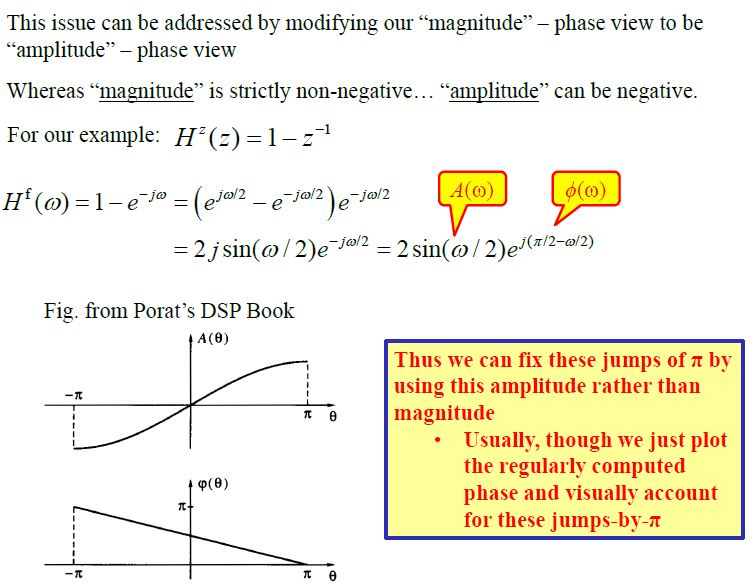
\includegraphics[width = 0.5\textwidth, frame]{Figures/FIR/linear_phase_example}
\caption{An example of linear phase system function}
\label{fig:FIR:linear_phase_example}
\end{figure}

\begin{itemize}

\item Notice that we let the amplitude $A(\omega_d)$ be positive and negative

    \begin{itemize}
        \item Not like MATLAB command \verb|abs| which compute the amplitude spectrum only using positive values
    \end{itemize}

\end{itemize}

In numerical computation using MATLAB, the angle spectrum will be shift by $\pi$, because MATLAB won't allow angle values be bigger then $\pi$.\\

An example is shown in \autoref{fig:FIR:linear_phase_example_matlab}, where every time the angle will be bigger then $\pm \pi$, MATLAB will do a shift by $2 \pi$, and this cause to make the jumps in the plots.\\

\begin{figure}[h]
\centering
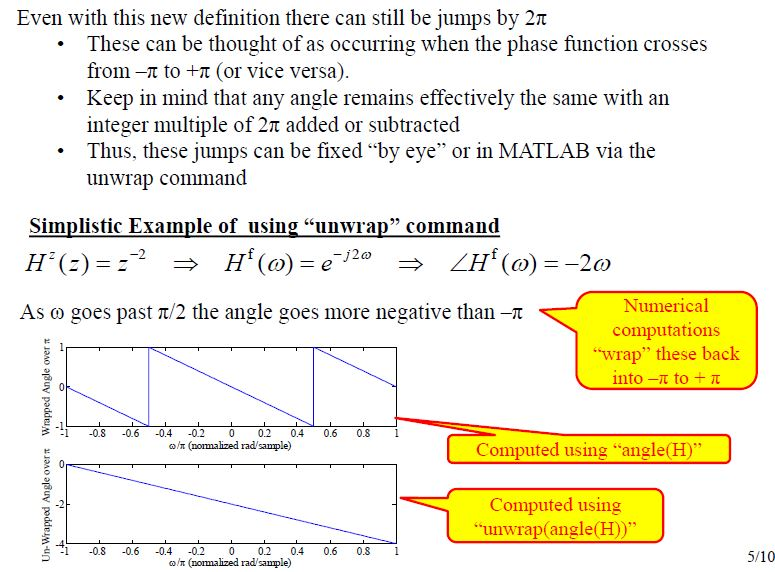
\includegraphics[width = 0.5\textwidth, frame]{Figures/FIR/linear_phase_example_matlab}
\caption{Wrapping Error for Phase Spectrum}
\label{fig:FIR:linear_phase_example_matlab}
\end{figure}

To fix the $2 \pi$ jumps, we can use the \verb|unwrap| command. But be aware, that \verb|unwrap| \tbi{fix only $ \pm 2 \pi$ jumps, and not the $ \pm \pi$ jumps}.
Notice for example that $\omega \, = \, 0$, $\phi(\omega) \, \neq \, 0$, and this is due to $\pi$ shift.\\

Handling $\pi$ shift is done theoretically or by hand.

\section{Linear Phase for FIR}

\subsection{Recap for FIR Equations}

\begin{figure}[h]
\centering
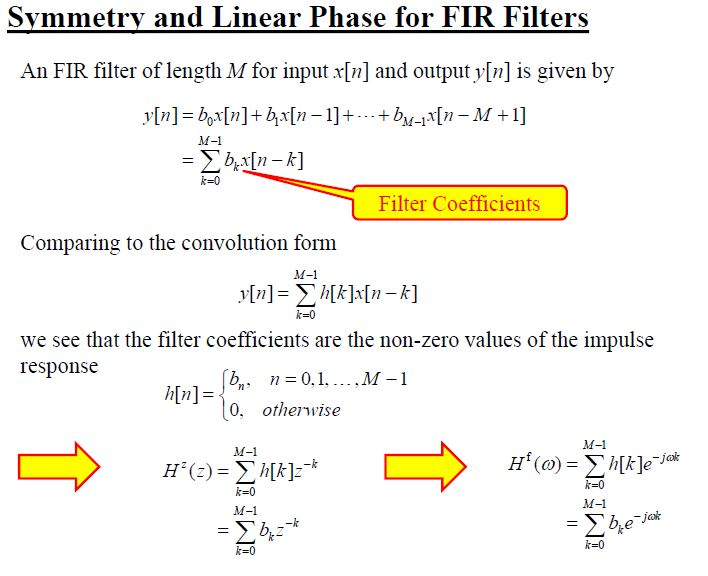
\includegraphics[width = 0.5\textwidth, frame]{Figures/FIR/FIR_Recap}
\caption{FIR Recap}
\label{fig:FIR:FIR_Recap}
\end{figure}

\begin{itemize}
    \item We have the difference equation of an FIR filter
    
    \item The impulse response $h[n]$ is composed from coefficients of the difference equation
    
    
    \item Filter coefficients are called \tbi{taps}
    
    
\end{itemize}


\subsection{Linear Phase definition for FIR}

We say that an FIR is linear in phase if its impulse response has symmetry

\begin{equation}
    h[k] \, = \, \pm \, h[M \, - \, 1 \, - \, k] \quad \text{for } k \, = \, 0 \, , \, 1 \, , \, \cdots \, , \, M \, - \, 1
\label{Eq:FIR:FIR_Symmetry_Impulse_Response}
\end{equation}

\begin{figure}[h]
\centering
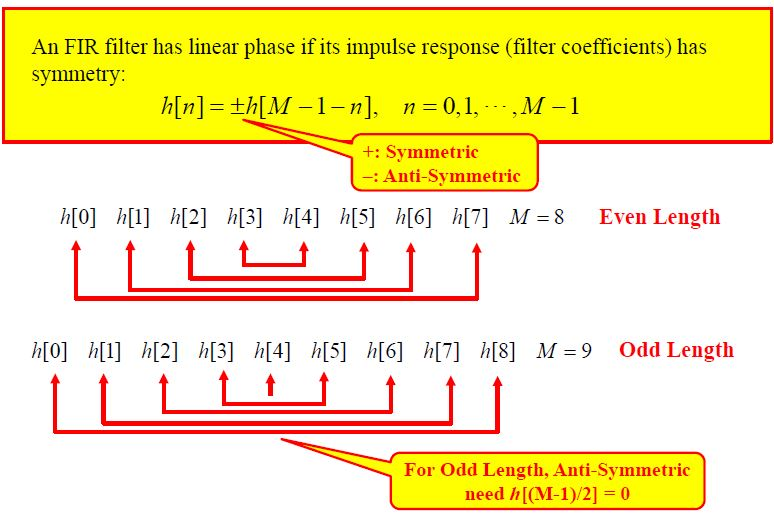
\includegraphics[width = 0.5\textwidth, frame]{Figures/FIR/FIR_Symmetry}
\caption{FIR Symmetry}
\label{fig:FIR:FIR_Symmetry}
\end{figure}

Notice that for odd length, we have a constraint for antisymmetric case. In the example of \autoref{fig:FIR:FIR_Symmetry}, if we have in symmetric case, we can say that $h[4] \, = \, h[4]$. But if we are in antisymmetric case, the only way we can say that $h[4] \, = \, -\,h[4]$ is if $h[4] \, = \, 0$, so we have some constraint to keep in mind in case of odd length antisymmetric case.\\

Using \autoref{Eq:FIR:FIR_Symmetry_Impulse_Response}, it can be shown that the frequency response $H_{\text{FIR}}(\omega_d)$ can be written in the form of an amplitude times an exponential having a linear phase. For a specific case demonstration, an example is shown in \autoref{fig:FIR:FIR_Symmetry_Proof_Example}, where the proof is done for the case of symmetric even length.

\begin{figure}[h]
\centering
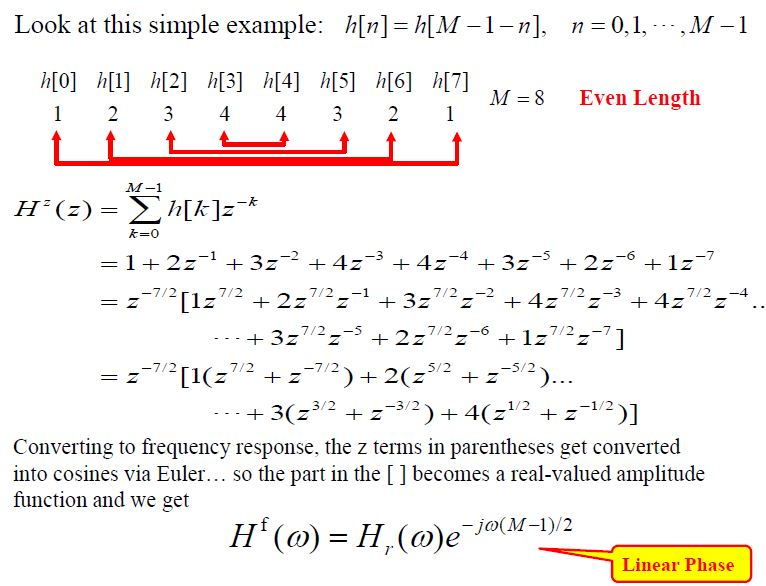
\includegraphics[width = 0.5\textwidth, frame]{Figures/FIR/FIR_Symmetry_Proof_Example}
\caption{FIR Linear Phase Proof by a example}
\label{fig:FIR:FIR_Symmetry_Proof_Example}
\end{figure}

\underline{General Formula:}\\


\begin{equation}
\begin{array}{rcl}
h[M \, - \, 1 \, - \, k] \, &=& \, \rightarrow \,  H_{\text{FIR}}(\omega_d) \, = \, \text{Amp}(\omega_d) \, \exp \left( \,  \displaystyle\frac{-j \, \omega_d \, (M \, - \, 1)}{2}  \,\right)  \\ \\
- \, h[M \, - \, 1 \, - \, k] \, &=& \, \rightarrow \,  H_{\text{FIR}}(\omega_d) \, = \, \text{Amp}(\omega_d) \, \exp \left( \,  \displaystyle\frac{-j \, \omega_d \, (M \, - \, 1)}{2}  \, + \, \displaystyle\frac{\pi}{2} \right)  \\ \\
\end{array}    
\end{equation}

For antisymmetric case, we have a shift of $ \displaystyle\frac{\pi}{2} $ in the phase spectrum.

\subsection{Zero Pattern}

For a linear phase FIR filter, we get an inverse of zero in addition to the initial one.

\subsection{Use case for Symmetric and Anti-symmetric}

Antisymmetric are note suited for LPF, because $H( \omega_d \, =\, 0) \, = \, 0$, which is not wanted in a LPF frequency response.

\section{Window Design Technique}

This method is not the commonly used one since it is not that effective, but it is a simple one and a good starting point.\\

In \autoref{fig:FIR:FIR_LPF_Sinc}, we have some LPF with some cut-off frequency to design. The impulse response is a sinc which is non-causal. The phase is linear.\\


\begin{figure}[h]
\centering
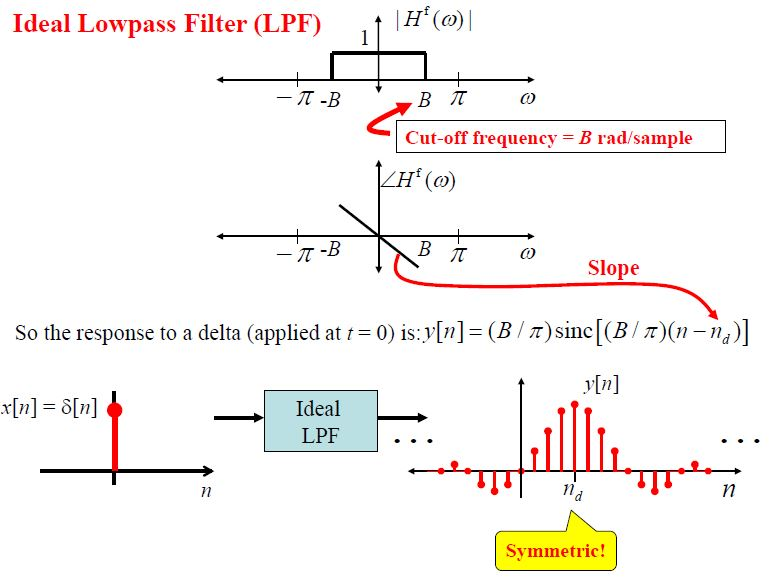
\includegraphics[width = 0.5\textwidth, frame]{Figures/FIR/FIR_LPF_Sinc}
\caption{LPF FIR}
\label{fig:FIR:FIR_LPF_Sinc}
\end{figure}

\underline{Design Key:} Usually we are interested that the phase is linear, but we don't care that much with its slope. We see later how we can achieve certain slope.\\

\newpage
The best way to make it causal is to simply truncate the values before 0, and also we truncate the symmetrical part which are after 0 to preserve the symmetry. The filter response after truncation is shown in \autoref{fig:FIR:FIR_window_method_truncation}.

\begin{figure}[h]
\centering
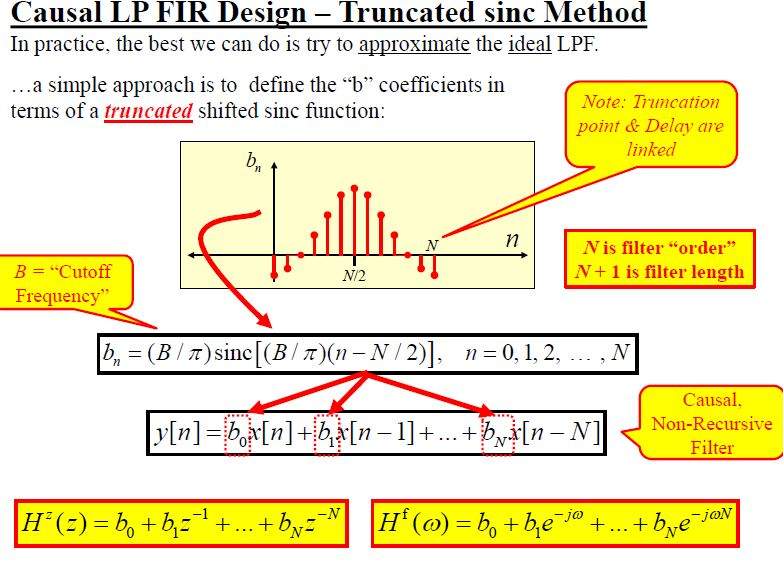
\includegraphics[width = 0.5\textwidth, frame]{Figures/FIR/FIR_window_method_truncation}
\caption{Truncation Method}
\label{fig:FIR:FIR_window_method_truncation}
\end{figure}

In this type of design to obtain a integer shift, we have to choose $N$ even.\\

An example is shown in \autoref{fig:FIR:FIR_window_method_example}.

\begin{figure}[h]
\centering
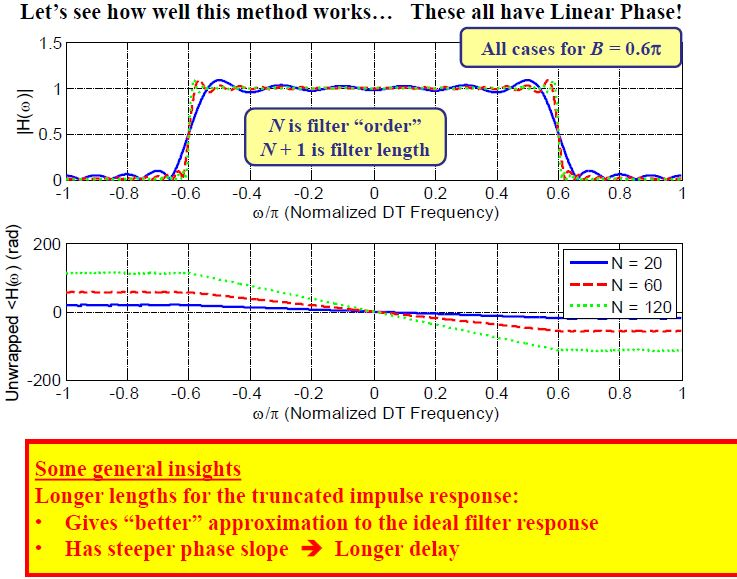
\includegraphics[width = 0.5\textwidth, frame]{Figures/FIR/FIR_window_method_example}
\caption{Truncation Method}
\label{fig:FIR:FIR_window_method_example}
\end{figure}


\begin{itemize}
    \item Notice that when the order $N$ increase, we have a more sharper transition bandwidth.
        
        \begin{itemize}
            \item This is true for any desing, and not only this particular desing
        \end{itemize}
    
    \item The downside of this is that we don't get to enhance the ripples at the edge of the pass band even when we increase the order
    
\end{itemize}

\newpage
Another example in dB scale is shown \autoref{fig:FIR:FIR_window_method_example_dB}.

\begin{figure}[h]
\centering
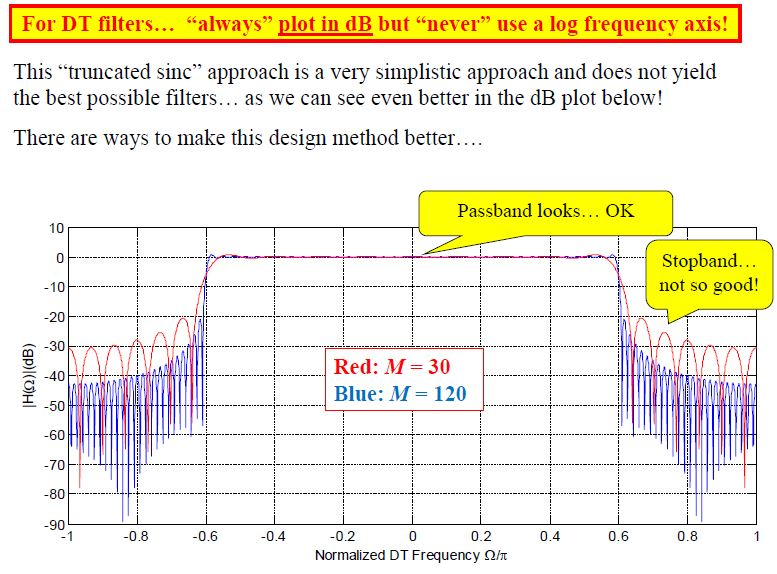
\includegraphics[width = 0.5\textwidth, frame]{Figures/FIR/FIR_window_method_example_dB}
\caption{Example of design in dB scale: stop band is not good at all}
\label{fig:FIR:FIR_window_method_example_dB}
\end{figure}

Even with the increase of the order, we have no a big difference the stop band attenuation levels between $M \, = \,30$ and $M \, = \, 120$.\\

\subsection{The usage of other window}

The problem of truncation is can simply formulated by multiplying the desired impulse response by some window, and hence we can use the knowledge of window types and tradeoff to controll the characteristic of the desired filter specification.

The lack of performance in the stop band seen in \autoref{fig:FIR:FIR_window_method_example_dB} is due to the sidelobes of rectangular window, which don't get lower even when we increase the length (hence the order of the filter).

Recall from Window analysis we have:

\begin{itemize}
    
\item Windows usually cause \tbi{smearing}

\item Usually we want some $h_{\text{desired}}[k]$, but we have is some windowed impulse due to windowing

\item Mathematically:
\begin{equation}
\begin{array}{rcl}
     h[k] \, &=& \, h_{\text{desired}}[k \, - \, k_d] \, \times \, w[k]  \\ \\
     H(\omega_d) \, &=& \, \displaystyle\frac{1}{2 \, \pi} \displaystyle\int\limits_{- \pi}^{+\pi} H_{\text{desired}}(\omega_d) \, W(\omega_d \, - \, \omega_0) \, d\omega_d
\end{array}    
\end{equation}

\item The sidelobes of the rectangular window will affect the ripples: the pass band (at the edge) and the stop band height

\item Whereas the mainlobe will controll the transition bandwidth of the filter

\end{itemize}


So as a design criteria:

\begin{itemize}
    \item Choose the window shape to get side lobes we want
    
    
    \item The length of the window control the transition band
    
\end{itemize}


\section{Frequency Sampling Technique}

The frequency sampling method rely on DFT computation, and taking finite frequency points at multiple of $\displaystyle\frac{2 \pi}{M}$. The steps are shown in \autoref{fig:FIR:FIR_frequency_sampling_method}


\begin{figure}[h]
\centering
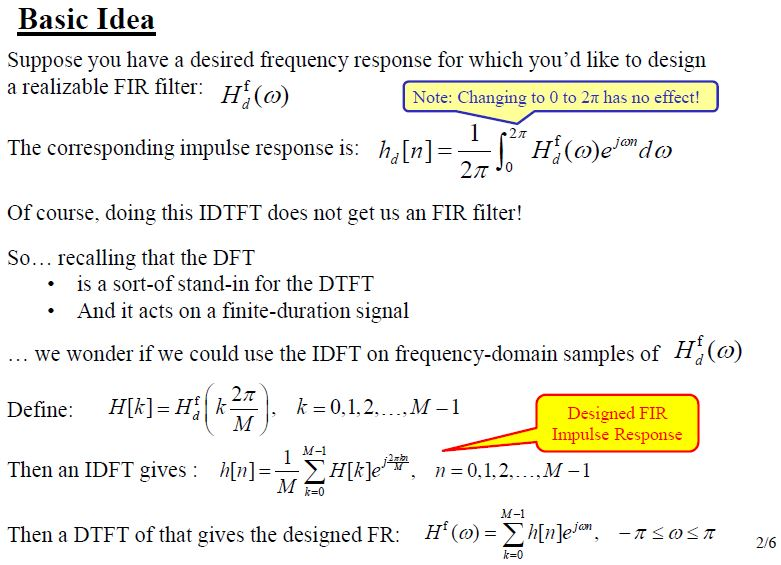
\includegraphics[width = 0.5\textwidth, frame]{Figures/FIR/FIR_frequency_sampling_method}
\caption{FIR using frequency sampling method}
\label{fig:FIR:FIR_frequency_sampling_method}
\end{figure}

\begin{itemize}
    

\item The period of integration in computing $h_{\text{desired}}[n]$ is changed to $0 \rightarrow \, 2 \pi$ instead of $- \pi \rightarrow +\pi$, in order to cover the frequency indices $k$ when computing the frequency response of the desired filter $H_{\text{des}}[k]$ at fininte frequency indices

\item Then we apply the inverse DFT to get some finite time domain signal which represent the desired filter (causal and finite)

\item As a check, we apply the DTFT again to the computed impulse response to check the filter


\end{itemize}

Summary results are shown in \autoref{fig:FIR:FIR_frequency_sampling_results}.

\begin{figure}[h]
\centering
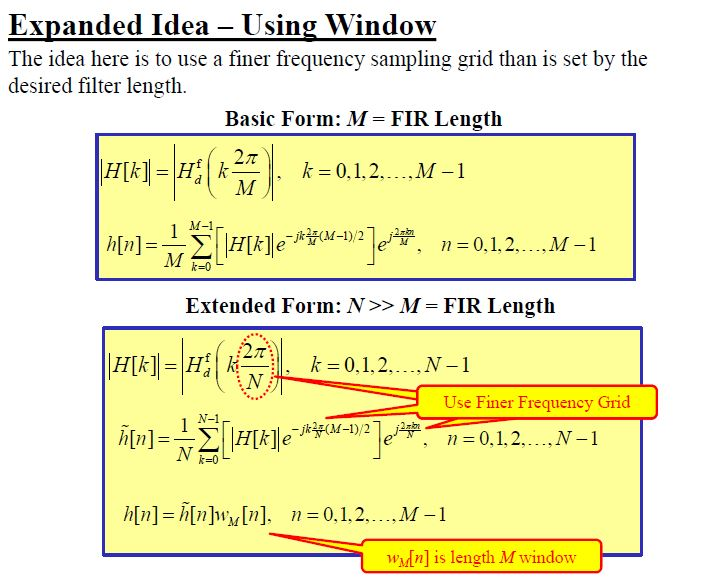
\includegraphics[width = 0.5\textwidth, frame]{Figures/FIR/FIR_frequency_sampling_results}
\caption{FIR using frequency sampling results}
\label{fig:FIR:FIR_frequency_sampling_results}
\end{figure}

\begin{itemize}

\item Usually we have $|H[k]|$ are specified

\item To ensure a linear phase, we add the term $e^{-j \, k \, \frac{2 \pi}{M} \, \left( \, \frac{M \, - \, 1}{2} \, \right) }$

\item The term $e^{j \, \frac{2 \pi k \, n}{M}}$ is from  the inverse DFT process

\item To enhance the design, more frequency sampling points $N >> \, M$ are taken

    \begin{itemize}
        \item But this give us a filter bigger then the desired
        
        \item That's why we multiply the $h_d[n]$ by a window
    \end{itemize}

\end{itemize}

Illustration using MATLAB shown in \autoref{fig:FIR:FIR_frequency_sampling_matlab}

\begin{figure}[h]
\centering
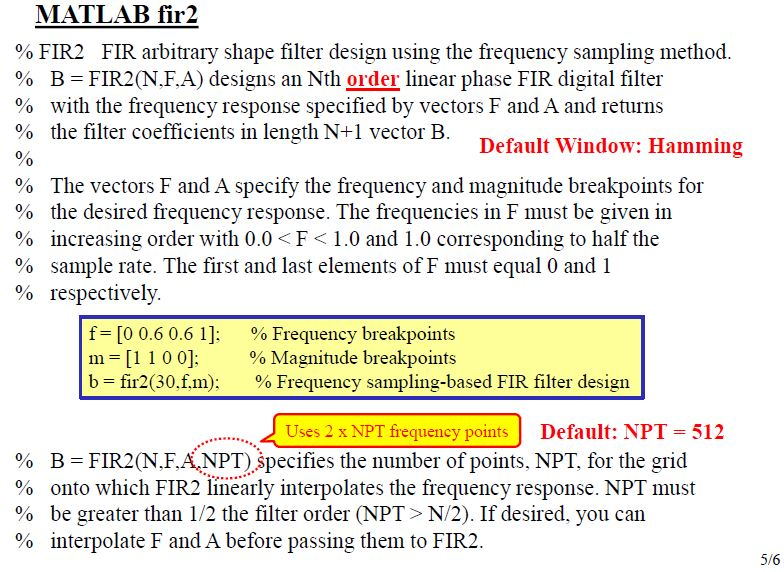
\includegraphics[width = 0.5\textwidth, frame]{Figures/FIR/FIR_frequency_sampling_matlab}
\caption{FIR using frequency sampling results}
\label{fig:FIR:FIR_frequency_sampling_matlab}
\end{figure}


\begin{itemize}
    \item $N$ is the order
    
    \item By default, number of frequency points is $2 \, \times \, 512$
    
    \item \verb|fir2| can make arbitrary (some special effect) in some frequency bands, unlike \verb|fir1|
    
    \item \verb|f| is inputed as a normalized vector in units of $\pi$, and \verb|m| is the desired magnitude
    
        \begin{itemize}
            \item In the example of \autoref{fig:FIR:FIR_frequency_sampling_matlab}, from $0 \rightarrow -0.6$, we have our passband since \verb|m| is 1 in this region
        \end{itemize}
    
\end{itemize}

\newpage
\section{Optimum Equiripple}

\begin{figure}[h]
\centering
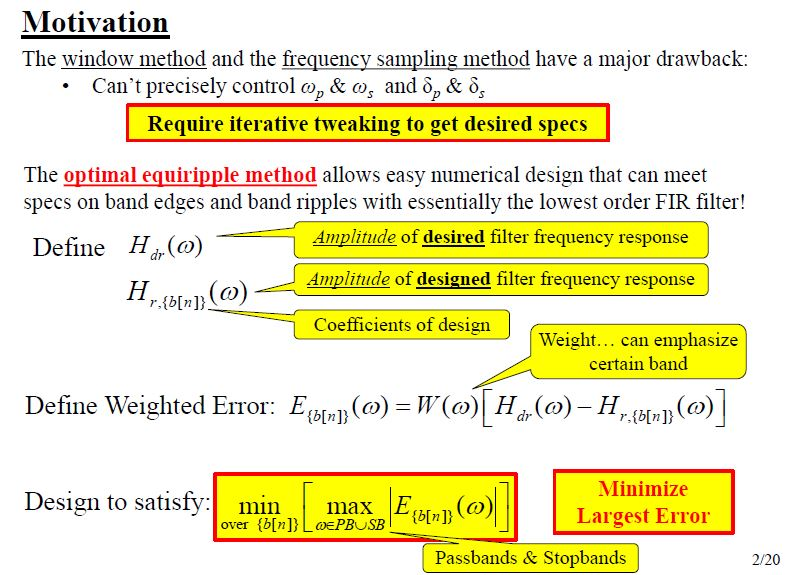
\includegraphics[width = 0.5\textwidth, frame]{Figures/FIR/FIR_optimum_equiripple}
\caption{FIR using Optimum Equiripple Method}
\label{fig:FIR:FIR_optimum_equiripple}
\end{figure}

\begin{itemize}

\item It was proposed by Parcs and McCellan in 1972, and implemented in FORTRAN

\item Drawback of previous designed methods: need to keep iterating to get the specs of the filter, and even after finishing iterating we won't get them all

\item The design criteria: minimize the largest error between the desired filter and the designed filter

    \begin{itemize}
        \item $H_{r \, , \, b[n]}$: in the designed filter, we explicitly show the coefficient $b[n]$ because there will be used using the design process
        
        \item $\max_{\omega \in PB \cup SB}$: maximize over all the pass band and the stop band $\leftrightarrow$ we don't care what happen in the transition band
        
    \end{itemize}


\end{itemize}

\subsection{MATLAB Example}


\begin{figure}[h]
\centering
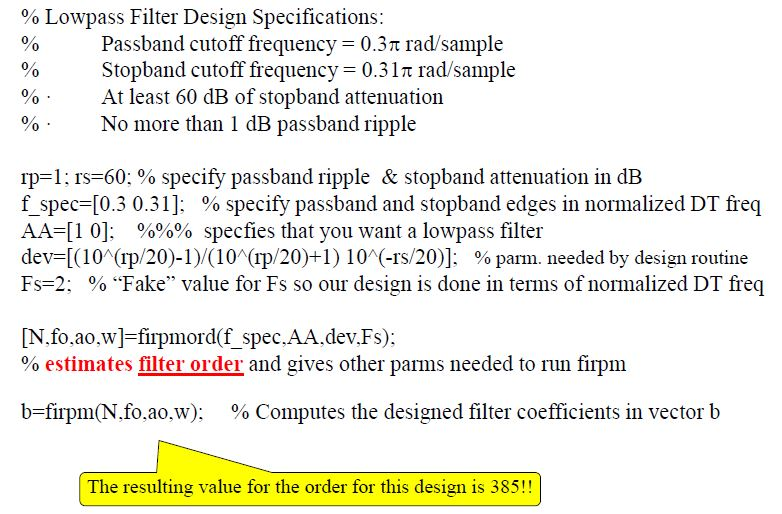
\includegraphics[width = 0.5\textwidth, frame]{Figures/FIR/FIR_optimum_equiripple_matlab_example}
\caption{FIR using Optimum Equiripple: A MATLAB Example}
\label{fig:FIR:FIR_optimum_equiripple_matlab_example}
\end{figure}


\begin{itemize}

\item First we are specifying the ripples in the pass band and the stop band $\leftrightarrow$ \verb|rp| and  \verb|rs|

\item Then we set the cuttoff frequencies \tbi{without the $\pi$} (the range goes from $0 \rightarrow 1$), this how MATLAB expects the frequencies

\item The sampling rate $F_s \, = \, 2$: we choose this value because usually we expect the range of frequencies from $0 \rightarrow \displaystyle\frac{F_s}{2}$.\\

If $F_s \, = \, 2 \rightarrow \,\displaystyle\frac{F_s}{2} \, = \, 1$, which corresponds to the range of the actual frequencies

    \begin{itemize}
        \item If we want to desing some pyhsical frequencies in Hz, we need to know the actual sampling rate in hz also.\\
        
        As an example: \verb|f-spec = [pass = 1000 , stop = 5000 Hz]| and $F_s \, = \, 40$KHz
    \end{itemize}

\item The \verb|dev| parameters is for the ripples $\delta_p$ and $\delta_s$: we convert them into linear scale

    \begin{itemize}
        \item Notice the - singe in front of \verb|rs| in the \verb|dev| variable: this is because it is an attenuation
    \end{itemize}


\end{itemize}

\subsection{Revisiting the Optimum Equiripple}

\todo{FIR Design}: To redo this section later.\\

In a broad view (this is from Dr Barry Veen), the optimum equiripple design consists of:

\begin{itemize}
    \item An objective function: a minimax criterion, where minimize over the coefficient of the FIR filter, the max absolute error between the desired (ideal) and the designed (actual)
    
    \item Take for example 1 form of the linear phase FIR (all of the contains cos terms)
    
    \item Use Chebychev polynomial (approximation theory), alternation theorem for the error, then Remez exchange algorithm, all of these methods are grouped under the name Parks-McCellan algorithm, which have used these mathematical tools to form fast, flexible FIR design method
    
    \item Unlike the previous 2 methods (window method and frequency sampling), the ripples in the pass and stop band were the same, but in some application we may have some different tolerance.
    
    The equiripple method can give us different tolerance, but in the expense of having equiripple oscillations (so not perfectly flat as before in window method and frequency sampling)
    
    
\end{itemize}